\documentclass[tikz, border=2pt]{standalone}
\usepackage{tikz}
\usepackage{pgfplots}
\usetikzlibrary{decorations.pathreplacing,calc}
\begin{document}
    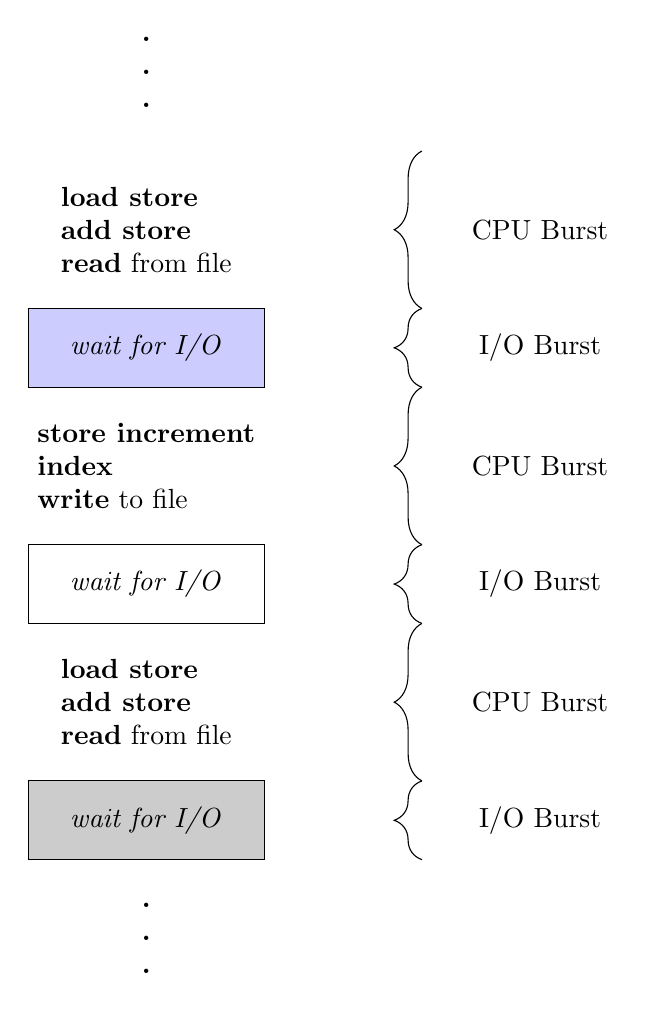
\begin{tikzpicture}
        \coordinate (io1) at (0,1.5);
        \coordinate (io2) at (0,4.5);
        \coordinate (io3) at (0,7.5);

        \node [align=center] at (0,0) {\textbf{.}\\\textbf{.}\\\textbf{.}};
        \draw [fill=black!20] (-1.5,1) rectangle (1.5,2);
        \node at (io1) {\textit{wait for I/O}};
        \node [align=left] at (0,3) {\textbf{load store}\\\textbf{add store}\\\textbf{read} from file};

        \draw (-1.5,4) rectangle (1.5,5);
        \node at (io2) {\textit{wait for I/O}};
        \node [align=left] at (0,6) {\textbf{store increment}\\\textbf{index}\\\textbf{write} to file};

        \draw [fill=blue!20] (-1.5,7) rectangle (1.5,8);
        \node at (io3) {\textit{wait for I/O}};
        \node [align=left] at (0,9) {\textbf{load store}\\\textbf{add store}\\\textbf{read} from file};

        \node [align=center] at (0,11) {\textbf{.}\\\textbf{.}\\\textbf{.}};

        \foreach \y in {1.5,4.5,7.5} {
            \draw[decorate,decoration={brace,amplitude=10pt},shift={(3,0)}] (0.5,\y-0.5) -- (0.5,\y+0.5);
            \draw[decorate,decoration={brace,amplitude=10pt},shift={(3,1.5)}] (0.5,\y-1) -- (0.5,\y+1);
            \node at (5, \y) {I/O Burst};
            \node at (5, \y+1.5) {CPU Burst};
        }
    \end{tikzpicture}
\end{document}